% This is the Reed College LaTeX thesis template. Most of the work
% for the document class was done by Sam Noble (SN), as well as this
% template. Later comments etc. by Ben Salzberg (BTS). Additional
% restructuring and APA support by Jess Youngberg (JY).
% Your comments and suggestions are more than welcome; please email
% them to cus@reed.edu
%
% See http://web.reed.edu/cis/help/latex.html for help. There are a
% great bunch of help pages there, with notes on
% getting started, bibtex, etc. Go there and read it if you're not
% already familiar with LaTeX.
%
% Any line that starts with a percent symbol is a comment.
% They won't show up in the document, and are useful for notes
% to yourself and explaining commands.
% Commenting also removes a line from the document;
% very handy for troubleshooting problems. -BTS

% As far as I know, this follows the requirements laid out in
% the 2002-2003 Senior Handbook. Ask a librarian to check the
% document before binding. -SN

%%
%% Preamble
%%
% \documentclass{<something>} must begin each LaTeX document
\documentclass[12pt,twoside]{reedthesis}
% Packages are extensions to the basic LaTeX functions. Whatever you
% want to typeset, there is probably a package out there for it.
% Chemistry (chemtex), screenplays, you name it.
% Check out CTAN to see: http://www.ctan.org/
%%
\usepackage{graphicx,latexsym}
\usepackage{amsmath}
\usepackage{amssymb,amsthm}
\usepackage{longtable,booktabs,setspace}
\usepackage{chemarr} %% Useful for one reaction arrow, useless if you're not a chem major
\usepackage[hyphens]{url}
% Added by CII
\usepackage{hyperref}
\usepackage{lmodern}
\usepackage{float}
\floatplacement{figure}{H}
% End of CII addition
\usepackage{rotating}

% Next line commented out by CII
%%% \usepackage{natbib}
% Comment out the natbib line above and uncomment the following two lines to use the new
% biblatex-chicago style, for Chicago A. Also make some changes at the end where the
% bibliography is included.
%\usepackage{biblatex-chicago}
%\bibliography{thesis}


% Added by CII (Thanks, Hadley!)
% Use ref for internal links
\renewcommand{\hyperref}[2][???]{\autoref{#1}}
\def\chapterautorefname{Chapter}
\def\sectionautorefname{Section}
\def\subsectionautorefname{Subsection}
% End of CII addition

% Added by CII
\usepackage{caption}
\captionsetup{width=5in}
% End of CII addition

% \usepackage{times} % other fonts are available like times, bookman, charter, palatino

% Syntax highlighting #22

% To pass between YAML and LaTeX the dollar signs are added by CII
\title{My Final College Paper}
\author{Your R. Name}
% The month and year that you submit your FINAL draft TO THE LIBRARY (May or December)
\date{May 20xx}
\division{Mathematics and Natural Sciences}
\advisor{Advisor F. Name}
\institution{Reed College}
\degree{Bachelor of Arts}
%If you have two advisors for some reason, you can use the following
% Uncommented out by CII
% End of CII addition

%%% Remember to use the correct department!
\department{Mathematics}
% if you're writing a thesis in an interdisciplinary major,
% uncomment the line below and change the text as appropriate.
% check the Senior Handbook if unsure.
%\thedivisionof{The Established Interdisciplinary Committee for}
% if you want the approval page to say "Approved for the Committee",
% uncomment the next line
%\approvedforthe{Committee}

% Added by CII
%%% Copied from knitr
%% maxwidth is the original width if it's less than linewidth
%% otherwise use linewidth (to make sure the graphics do not exceed the margin)
\makeatletter
\def\maxwidth{ %
  \ifdim\Gin@nat@width>\linewidth
    \linewidth
  \else
    \Gin@nat@width
  \fi
}
\makeatother

%Added by @MyKo101, code provided by @GerbrichFerdinands

\renewcommand{\contentsname}{Table of Contents}
% End of CII addition

\setlength{\parskip}{0pt}

% Added by CII

\providecommand{\tightlist}{%
  \setlength{\itemsep}{0pt}\setlength{\parskip}{0pt}}

\Acknowledgements{
I want to thank a few people.
}

\Dedication{
You can have a dedication here if you wish.
}

\Preface{
This is an example of a thesis setup to use the reed thesis document class
(for LaTeX) and the R bookdown package, in general.
}

\Abstract{
\hypertarget{abstract}{%
\chapter{Abstract}\label{abstract}}

The preface pretty much says it all.

\par

Second paragraph of abstract starts here.
}

% End of CII addition
%%
%% End Preamble
%%
%
\begin{document}

% Everything below added by CII
  \maketitle

\frontmatter % this stuff will be roman-numbered
\pagestyle{empty} % this removes page numbers from the frontmatter
  \begin{acknowledgements}
    I want to thank a few people.
  \end{acknowledgements}
  \begin{preface}
    This is an example of a thesis setup to use the reed thesis document class
    (for LaTeX) and the R bookdown package, in general.
  \end{preface}
  \hypersetup{linkcolor=black}
  \setcounter{tocdepth}{2}
  \tableofcontents

  \listoftables

  \listoffigures
  \begin{abstract}
    \hypertarget{abstract}{%
    \chapter{Abstract}\label{abstract}}
    
    The preface pretty much says it all.
    
    \par
    
    Second paragraph of abstract starts here.
  \end{abstract}
  \begin{dedication}
    You can have a dedication here if you wish.
  \end{dedication}
\mainmatter % here the regular arabic numbering starts
\pagestyle{fancyplain} % turns page numbering back on

\hypertarget{introduction}{%
\chapter*{Introduction}\label{introduction}}
\addcontentsline{toc}{chapter}{Introduction}

Pronouns are small words used in place of nouns in sentences (``Pronoun,'' 2020). Gendered pronouns are a type of pronoun that identifies the subject's gender when used (``Preferred gender pronoun,'' 2019). For example, in the sentence ``she walks the dog,'' she is the third person pronoun that replaces the subject's name. In English, the most common pronouns are ``she,'' ``they,'' and ``he.'' It is important to note that ``they'' is widely recognized as both a singular and plural pronoun (``They,'' 2019).

Gendered pronouns are especially important for transgender and non-binary individuals, since their apperance and gender may not match cisnormative expectations.

\hypertarget{litreview}{%
\chapter{Literature Review}\label{litreview}}

Gendered pronouns.

\hypertarget{methods}{%
\chapter{Methods}\label{methods}}

\emph{Participants}

477 undergraduate students from Reed College in Portland, Oregon participated in an online survey about ``attitudes towards gendered pronouns.'' Participants were recruited through online advertisements and posters around campus. Notably, this sample is around one-third of the undergraduate student body. Data colleciton was conducted over a two month period, starting in Febuary 2020. It should be noted that the global pandemic that occured in early 2020 shortened our opportunity to collect data.

\hypertarget{results}{%
\chapter{Results}\label{results}}

\hypertarget{demographics}{%
\section{Demographics}\label{demographics}}

I collected gender-related demographic data by asking participants to write in their gender identity and answer a series of yes/no questions: ``Are you cisgender?,'' ``Are you transgender?,'' and ``Is your gender non-binary?'' Answering yes on one question did not force the participants to answer no on others---this treated gender identity as a collection of separate, related labels that participants may or may not identify with simultaneously. Responses for the write-in question were qualitatively coded by me.

Overall, 317 participants identified as cisgender, 81 identified as transgender, and 141 identified their gender as non-binary. It is important to note that there is overlap among these groups. 63 participants said they were transgender and non-binary, 16 participants said they were cisgender and non-binary, and 1 participant said they were cisgender, transgender, and non-binary.

The most common gender themes were woman (\emph{N} = 220), man (\emph{N} = 120), non-binary (\emph{N} = 94), cisgender (\emph{N} = 36), transgender (\emph{N} = 26), questioning (\emph{N} = 24), masculine (\emph{N} = 18), agender (\emph{N} = 15), genderfluid (\emph{N} = 15), and queer (\emph{N} = 8).

\hypertarget{experiences-with-misgendering}{%
\section{Experiences with Misgendering}\label{experiences-with-misgendering}}

Similar to McLemore (2015), we had participants report how frequently they were misgendered and how stigmatized misgendering made them feel. However, unlike McLemore (2015), we administered these questions to cisgender people as well. Independent t-tests were used to compare the cisgender and non-cisgender participants. Non-cisgender participants (\emph{M} = NaN, \emph{SD} = NA) reported being misgendered more frequently than cisgender participants (\emph{M} = NaN, \emph{SD} = NA), \emph{t}(231) = 21.6, \emph{p} \textless{} 0.001.
Non-cisgender participants (\emph{M} = NaN, \emph{SD} = NA) also reported feeling more stigmatized when misgendered than than cisgender participants (\emph{M} = NaN, \emph{SD} = NA), \emph{t}(261) = 12.9, \emph{p} \textless{} 0.001.
\begin{table}

\caption{\label{tab:unnamed-chunk-1}Misgendering frequency for non-cisgender and cisgender participants}
\centering
\begin{tabular}[t]{l|r|r}
\hline
“How often do people ‘misgender’ you?” & Non-cisgender (\%) & Cisgender (\%)\\
\hline
Never & 6.4 & 68.8\\
\hline
Rarely & 14.0 & 24.9\\
\hline
Sometimes & 30.6 & 4.7\\
\hline
Often & 44.6 & 1.3\\
\hline
Always & 4.5 & 0.3\\
\hline
\end{tabular}
\end{table}
\begin{table}

\caption{\label{tab:unnamed-chunk-2}Felt stigma when misgendered for non-cisgender and cisgender participants}
\centering
\begin{tabular}[t]{l|r|r}
\hline
“I feel stigmatized (looked down upon)when I am misgendered.” & Non-cisgender (\%) & Cisgender (\%)\\
\hline
Not at all & 12.2 & 68.5\\
\hline
Slightly & 20.5 & 12.0\\
\hline
Somewhat & 28.2 & 13.4\\
\hline
Considerably & 18.6 & 4.0\\
\hline
Very & 20.5 & 2.2\\
\hline
\end{tabular}
\end{table}
Pearson's Chi-squared tests were used to compare the misgendering frequency observed in McLemore (2015) to the non-cisgender participants in the present study.
There were significant differences when compared to both the study 1 population, \emph{X2} (4, \emph{N} = 864) = 178.18, \emph{p} = 0, and the study 2 population, \emph{X2} (4, \emph{N} = 902) = 228.69, \emph{p} = 0.

McLemore (2015) performed a one-way ANOVA ``to compare differences among three gender groups (transgender men, transgender women, and genderqueer)'' in misgendering frequency and felt stigma when misgendered.
Because I took a different approach to collecting gender-related demographic data, I elected to perform a factorial ANOVA comparing endorsement of several endorsed identities on misgendering frequency and felt stigma.

There were multiple significant effects of identity endorsement on misgendering frequency.
Cisgender, \emph{F}(1, 464) = 702.04, \emph{p} \textless{} 0.001,
transgender, \emph{F}(1, 464) = 21.3, \emph{p} \textless{} 0.001,
and non-binary identity, \emph{F}(1, 464) = 40.59, \emph{p} \textless{} 0.001, all demonstrated significant effects.
There was no significant effect in women (\emph{p} = 0.11) or men (\emph{p} = 0.08) alone.
However, there was a significant effect in transgender women, \emph{F}(1, 464) = 11.76, \emph{p} \textless{} 0.001.
There was not a significant effect in transgender men (\emph{p} = 0.37).
There was also a significant effect in non-binary women , \emph{F}(1, 464) = 11.76, \emph{p} = 0.004,
but not in non-binary men (\emph{p} = 0.296).

There were also multiple sigificant effects of identity endorsement on felt stigma when misgendered.
Cisgender, \emph{F}(1, 422) = 210.75, \emph{p} \textless{} 0.001,
and transgender , \emph{F}(1, 422) = 39.81, \emph{p} \textless{} 0.001, identities demonstrated significant effects.
However, non-binary (\emph{p} = 0.15) identity did not show a significant effect.
Neither men (\emph{p} = 0.51) nor women (\emph{p} = 0.38) alone showed significant effects, nor did trans women (\emph{p} = 0.69).
However, trans men, \emph{F}(1, 422) = 7.41, \emph{p} \textless{} 0.001, demonstrated a significant effect.
Neither non-binary men (\emph{p} = 0.77) nor non-binary women (\emph{p} = 0.43) demonstrated a significant effect.

Unlike McLemore (2015), I also collected participants pronouns. This allowed me to perform a factorial ANOVA with a follow-up Tukey test to examine pronouns, independent of gender, had an effect on misgendering frequency. I will finish this paragraph later lol once i figure out if it's actually relevant or not lol.

\hypertarget{gender-congruence}{%
\section{Gender Congruence}\label{gender-congruence}}

Kozee, Tylka, \& Bauerband (2012) developed the TCS (Transgender Congruence Scale) to measure transgender individuals' relationship and comfort between their inner gender identity, physical appearance, and social experience of gender. In this study, the TCS was administered to cisgender participants as well.

A single sample t-test revealed that non-cisgender participants (\emph{M} = 41.39, \emph{SD} = 8.01) scored lower on the TCS than cisgender participants (\emph{M} = 46.36, \emph{SD} = 6.44), \emph{t}(348.89) = -20.04, \emph{p} \textless{} 0.001.

A factorial ANOVA demonstrated significant effects of cisgender, \emph{F}(1, 267) = 352.4, \emph{p} \textless{} 0.001,
and non-binary identification, \emph{F}(1, 267) = 10.83, \emph{p} \textless{} 0.001,
but not of transgender identification (\emph{p} = 0.71).
There were also no significant effects in men (\emph{p} = 0.46), women (\emph{p} = 0.16), trans men (\emph{p} = 0.56), trans women (\emph{p} = 0.64), non-binary men (\emph{p} = 0.28), and non-binary women (\emph{p} = 0.33).

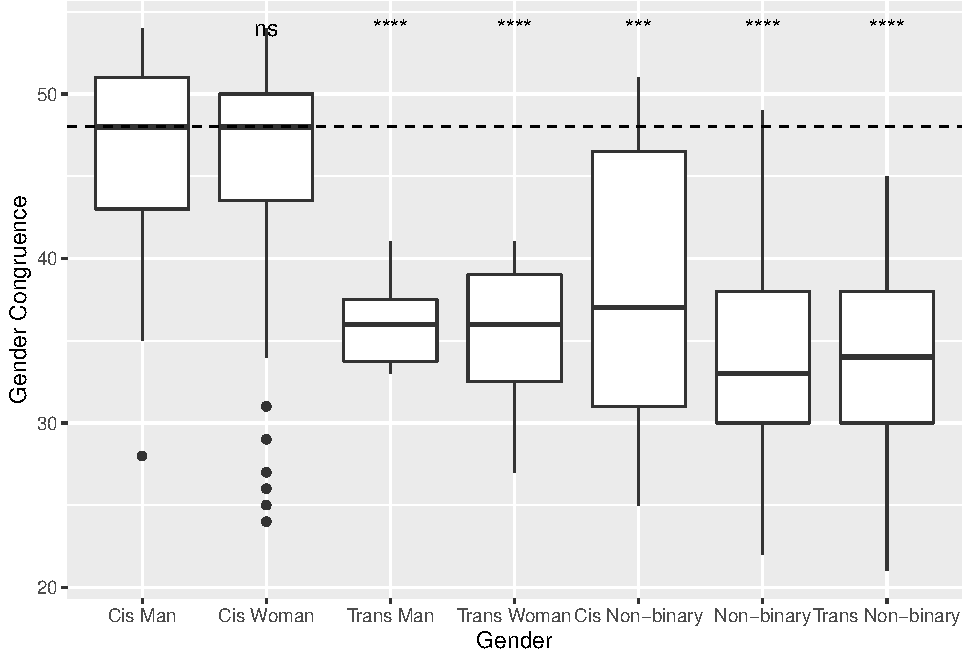
\includegraphics{thesis_files/figure-latex/congruence_graph-1.pdf}

\hypertarget{transgender-inclusive-behaviors}{%
\section{Transgender Inclusive Behaviors}\label{transgender-inclusive-behaviors}}

Kattari, O'Connor, \& Kattari (2018) developed the Transgender Inclusive Behavior Scale (TIBS) as a method of quantifying the number of behaviors that may support and include transgender people that one regularly does. Scores are a sum of responses on a series of five-point likert scales ranging from ``Never'' to ``Often.''

A single-sample t-test revealed that non-cisgender people (\emph{M} = 51.34, \emph{SD} = 9.14) reporting performing more inclusive behaviors than cisgender people (\emph{M} = 41.98, \emph{SD} = 9.26), \emph{t}(304.22) = 10.22, \emph{p} \textless{} 0.001.

A one-way ANOVA demonstrated that there was a significant effect of gender \emph{F}(6, 249) = 26.53, \emph{p} \textless{} 0.001.
A Tukey post-hoc comparison revealed that cisgender men (\emph{M} = 37.31, \emph{SD} = 8.92) do significantly fewer trans inclusive behaviors than cisgender women (\emph{M} = 44.43, \emph{SD} = 8.18), transgender men (\emph{M} = 55.91, \emph{SD} = 9.16), transgender women (\emph{M} = 50.58, \emph{SD} = 9.97), cisgender non-binary people (\emph{M} = 45.73, \emph{SD} = 8.18), non-binary people (\emph{M} = 49.26, \emph{SD} = 9.3), and transgender non-binary people (\emph{M} = 53.85, \emph{SD} = 7.71). Cisgender women do significantly fewer trans inclusive behaviors than transgender men, transgender women, non-binary people, and transgender non-binary people. Cisgender non-binary people also do fewer trans inclusive behaviors than transgender non-binary people.

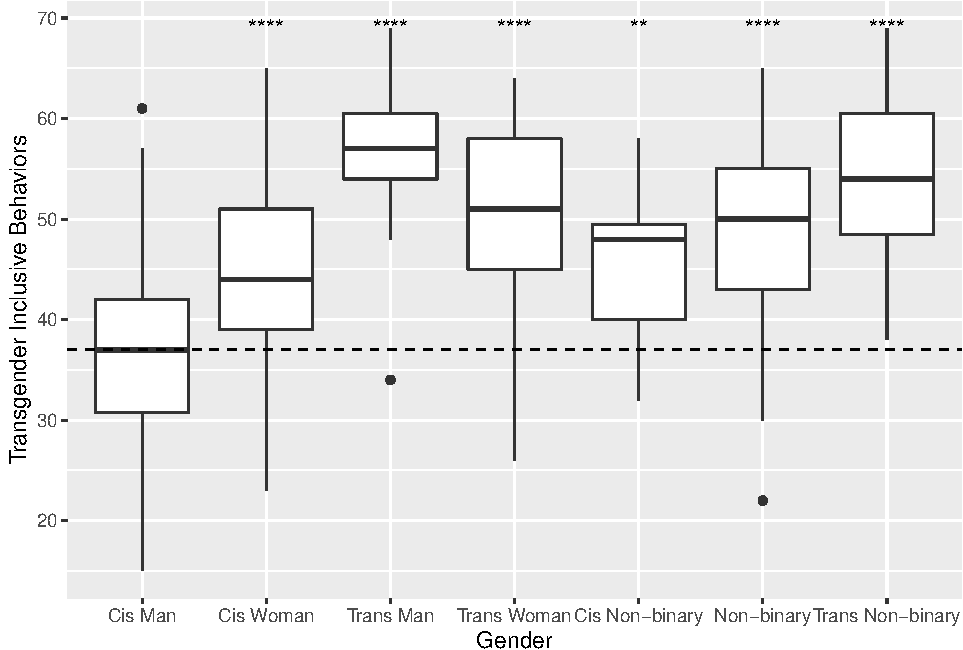
\includegraphics{thesis_files/figure-latex/incl_behavior_graph-1.pdf}

\hypertarget{pronouns}{%
\section{Pronouns}\label{pronouns}}

I administered a series of questions about comfort with and relationships towards gendered pronouns.

\hypertarget{discussion}{%
\chapter{Discussion}\label{discussion}}

So, we found some gendered pronouns.

\appendix

\backmatter

\hypertarget{references}{%
\chapter*{References}\label{references}}
\addcontentsline{toc}{chapter}{References}

\markboth{References}{References}

\noindent

\setlength{\parindent}{-0.20in}
\setlength{\leftskip}{0.20in}
\setlength{\parskip}{8pt}

\hypertarget{refs}{}
\leavevmode\hypertarget{ref-kattariDevelopmentValidationTransgender2018}{}%
Kattari, S. K., O'Connor, A. A., \& Kattari, L. (2018). Development and Validation of the Transgender Inclusive Behavior Scale (TIBS). \emph{Journal of Homosexuality}, \emph{65}(2), 181--196. \url{http://doi.org/10.1080/00918369.2017.1314160}

\leavevmode\hypertarget{ref-kozeeMeasuringTransgenderIndividuals2012}{}%
Kozee, H. B., Tylka, T. L., \& Bauerband, L. A. (2012). Measuring Transgender Individuals' Comfort With Gender Identity and Appearance: Development and Validation of the Transgender Congruence Scale. \emph{Psychology of Women Quarterly}, \emph{36}(2), 179--196. \url{http://doi.org/10.1177/0361684312442161}

\leavevmode\hypertarget{ref-mclemoreExperiencesMisgenderingIdentity2015}{}%
McLemore, K. A. (2015). Experiences with Misgendering: Identity Misclassification of Transgender Spectrum Individuals. \emph{Self and Identity}, \emph{14}(1), 51--74. \url{http://doi.org/10.1080/15298868.2014.950691}

\leavevmode\hypertarget{ref-PreferredGenderPronoun2019}{}%
Preferred gender pronoun. (2019). \emph{Wikipedia}.

\leavevmode\hypertarget{ref-Pronoun2020}{}%
Pronoun. (2020). \emph{Mirriam-Webster}.

\leavevmode\hypertarget{ref-They2019}{}%
They. (2019). \emph{Merriam-Webster.com}.


% Index?

\end{document}
